\documentclass[5pt]{article}
\usepackage{makeidx}
\usepackage{graphicx}
\usepackage{amsmath}
\usepackage{amssymb}
\usepackage{latexsym}
\renewcommand\refname{Referenze}
\usepackage[utf8x]{inputenc}
\usepackage{titlesec}
\usepackage{bm}
\usepackage{mathtools}
\usepackage[document]{ragged2e}
\titleformat{\section}{\huge\normalfont\bf}{\thesection.\hspace{5pt}}{5pt}{\vspace{1cm}}
\titleformat*{\subsection}{\Large\bfseries}
\usepackage[inner=3cm,outer=3cm]{geometry}

\makeindex

\begin{document}
\justify
\printindex
\Large{A.a. 2013-2014}
\vspace{10cm}
\begin{center}
\Huge\textbf{Diffusione Compton}
\end{center}

\vspace{2cm}
\begin{flushleft}
\textit{Gruppo \textsc{1}} \\
\medskip
Federico \textsc{Massa} \\ 
Marco \textsc{Montella}
\end{flushleft}



\newpage

\begin{abstract}
\justify
 

\end{abstract}
\bigskip

\section{Introduzione} \label{sec:intro}
Un fotone che attraversa un determinato materiale può interagire in vari modi a seconda della sua energia. A basse energie (ma superiori a quelle di estrazione degli elettroni atomici) domina l'effetto fotoelettrico. All'aumentare dell'energia l'effetto dominante diventa quello di diffusione Compton, la cui rappresentazione in diagramma di Feynman è mostrata in Fig. \ref{fig:feynman}. Ad energie ancora maggiori l'effetto dominante è quello di produzione di coppia elettrone-positrone. In Fig. \ref{fig:cross_sections} è mostrata la sezione d'urto totale, che comprende anche i piccoli contributi di produzione di coppia dovuta al campo degli elettroni ($\gamma e^- \rightarrow e^+ e^- \hspace{1 pt} e^-$) e le interazioni con il nucleo. 

\begin{figure}
\begin{center}
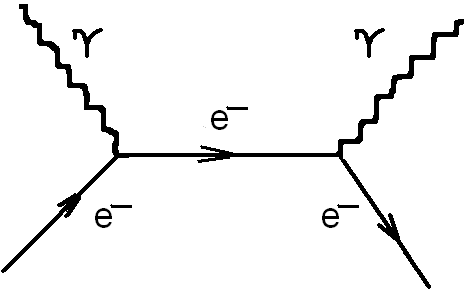
\includegraphics[scale=0.5]{feynman}
\caption{Diagramma di Feynman della diffusione Compton.}
\label{fig:feynman}
\end{center}
\end{figure}


\begin{figure}
\begin{center}
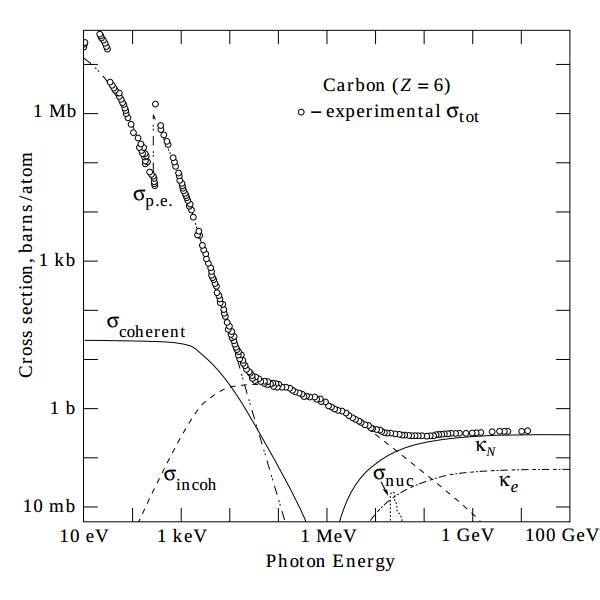
\includegraphics[scale=0.5]{cross_sections}
\caption{Grafico dei contributi alla sezione d'urto totale di interazione dei fotoni nel Carbonio.}
\label{fig:cross_sections}
\end{center}
\end{figure}

Scopo dell'esperimento è quello di studiare le caratteristiche della diffusione Compton verificando in particolare due relazioni caratteristiche. La prima è una relazione cinematica che lega l'energia del fotone diffuso all'angolo di diffusione ed è descritta dalla seguente equazione: \\

\begin{equation}
E'\ = \ \frac{E}{1+\frac{E}{m_e}\left(1-\cos{\theta}\right)}
\label{eq:en_ang}
\end{equation}

La seconda riguarda invece la sezione d'urto differenziale, che è descritta dalla \textit{formula di Klein Nishina}:

\begin{equation}
\frac{d\sigma}{d\Omega} = \frac{r_0 ^2}{2} \ P^2(E/m , \theta) \left[ P(E/m, \theta) + P^{-1} (E/m, \theta) -1 + cos^2(\theta)\right]
\label{eq:klein}
\end{equation}



\section{Apparato sperimentale} \label{sec:apparato}
\begin{figure}
\begin{center}
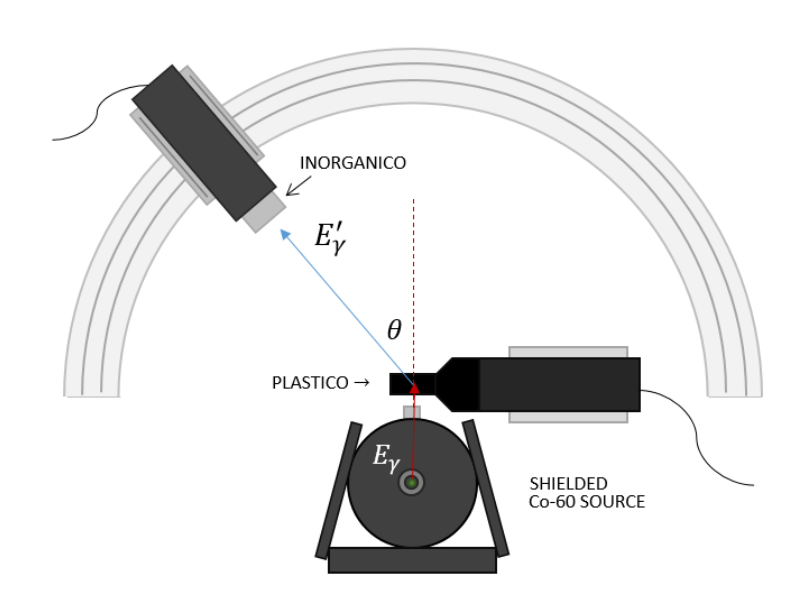
\includegraphics[scale=0.5]{Apparato2}
\caption{Apparato sperimentale. $\theta$ indica l'angolo di diffusione, $E_\gamma$ l'energia del fotone emesso dalla sorgente e $E'_\gamma$ l'energia del fotone diffuso.}
\label{fig:apparato}
\end{center}
\end{figure}



\subsection{Sorgente}
L'analisi della diffusione Compton è stata effettuata utilizzando una sorgente radioattiva di \textit{Co-60} di attività nominale a Maggio 2011 di $7.4 \cdot 10^7 Bq$, dalla quale, grazie alla conoscenza della vita media dell'elemento ($1925 \ d$), è stata ricavata l' attività al momento dell' inizio dell'esperimento ($01/04/2014$), che è risultata di $4.29 \cdot 10^7 Bq$. Alla fine dell'esperimento l'attività si stima essere diminuita di circa 1.5\%, ma le misure che richiedevano coerenza temporale sono state effettuate nel giro di un giorno, nel quale l'attività si è stimata essere variata solo dello 0.05\%, quantità trascurabile rispetto alle altre incertezze sperimentali.
L'elemento utilizzato è contraddistinto da due picchi di emissione di intensità approssimativamente uguale, con picchi centrati attorno ai valori $1173.228 \ keV$ e $1332.494 \ keV$. 
Si tratta di una sorgente adeguata per l'analisi dell'effetto Compton in quanto a tali energie esso è dominante rispetto agli altri effetti (Fig. \ref{fig:cross_sections}).

\subsection{Schermature e collimazione del fascio}
Con riferimento alla Fig. \ref{fig:apparato}, i fotoni emessi dalla sorgente sono schermati da un cilindro di piombo di spessore $10 \ cm$. Conoscendo la sezione d'urto Compton nel piombo\cite{PDG_lead}, è possibile calcolare la lunghezza di attenuazione, che risulta $3 \ cm$. Si stima dunque che con tale spessore di piombo solo il 4\% circa dei fotoni riesca a superare la schermatura. \\
Il fascio è collimato grazie a un'apertura praticata nel cilindro di piombo di diametro $0.8 \ cm$. Il collimatore può essere eventualmente tappato con un piccolo cilindro di piombo alla fine delle misure.

\subsection{Rivelatori}
La configurazione sperimentale tipica è rappresentata in Fig. \ref{fig:apparato}. I fotoni emessi dalla sorgente fuoriescono attraverso il collimatore e attraversano uno \textbf{scintillatore plastico} di spessore $2.5 \ cm$. 
Essendo l'interazione dominante in questo intervallo di energie l'effetto Compton, quando
l'interazione avviene il fotone viene deflesso di un certo angolo $\theta$ rispetto alla direzione di arrivo.
Questo può essere a sua volta rivelato da uno \textbf{scintillatore inorganico} al NaI, di sezione circolare di diametro $5.08 \ cm$.
Quest'ultimo è stato posizionato ad una distanza di $30 \ cm$ dallo scintillatore plastico.

\subsection{Goniometro}

Essendo lo scintillatore inorganico vincolato a muoversi su un arco di circonferenza, risulta di fondamentale importanza la misura della posizione angolare di quest'ultimo rispetto a uno zero che non deve necessariamente coincidere con il centro geometrico del fascio. \\
A questo scopo si è posizionato lo scintillatore plastico a circa $2 cm$ dall'estremità del collimatore e nel punto medio della congiungente degli estremi della guida dell'inorganico.
Abbiamo quindi posizionato un goniometro prestando attenzione al fatto che il centro si trovasse sulla verticale del punto di incontro tra l'asse del collimatore e il centro del plastico.
\'E legittimo supporre infatti che la maggior parte delle interazioni avvengano in un intorno di questo punto, le cui dimensioni sono determinate dalla larghezza del fascio. \\

\subsection{Elettronica}

L'uso di un \textit{oscilloscopio} permette di analizzare le caratteristiche qualitative e quantitative dei segnali analogici e digitali in uscita dalla catena elettronica. Il segnale analogico proveniente dallo scintillatore plastico risulta essere di durata pari a qualche decina di $ns$, mentre quello proveniente dallo scintillatore inorganico di qualche $\mu s$. 

Un'opportuna catena elettronica si occupa di svolgere le funzioni necessarie al corretto svolgimento dell'esperimento, che sono: \\

\begin{itemize}
\item Alimentazione dei fotomoltiplicatori che convertono il segnale luminoso proveniente dagli scintillatori in un segnale elettronico.
\item Digitalizzazione del segnale proveniente dallo scintillatore plastico. Questa avviene
quando il segnale analogico proveniente dallo stesso supera una data tensione di soglia. Questa funzione è svolta dal \textit{modulo di discriminazione}, con il quale si può anche impostare la durata del segnale digitale in uscita.
\item Amplificazione e inversione del segnale proveniente dallo scintillatore inorganico. Il segnale in uscita è positivo e ha una durata di ordine $1 \ \mu s$. Il guadagno può essere regolato con un opportuno potenziometro e l'amplificatore ha anche la possibilità di ricevere un segnale di \textit{gate}, come verrà descritto successivamente. !!! CHECK
\item Digitalizzazione del segnale proveniente dallo scintillatore inorganico. La maniera corretta di eseguire questa operazione verrà descritta poco più avanti.
\item Messa in tempo dei due rivelatori. Questa operazione necessita di \textit{moduli di coincidenza} che restituiscano un segnale ogniqualvolta entrambi i rivelatori lo restituiscono e di \textit{scatole di ritardo} in grado di variare lo sfasamento temporale dei segnali provenienti dai due rivelatori.
\item Conteggio dei segnali provenienti dai singoli rivelatori o del numero di segnali in coincidenza. Questo è realizzato con opportuni \textit{moduli multiscaler}.
\item Invio del segnale analogico proveniente dallo scintillatore inorganico ad una scheda di acquisizione
\end{itemize}

Come si è detto, la digitalizzazione del segnale proveniente dallo scintillatore inorganico richiede una procedura differente rispetto a quella dello scintillatore plastico. Questo è dovuto principalmente alla differente ampiezza e durata del segnale analogico. L'operazione è stata effettuata come segue (Fig. \ref{fig:dual_1}): \\

\begin{figure}
\begin{center}
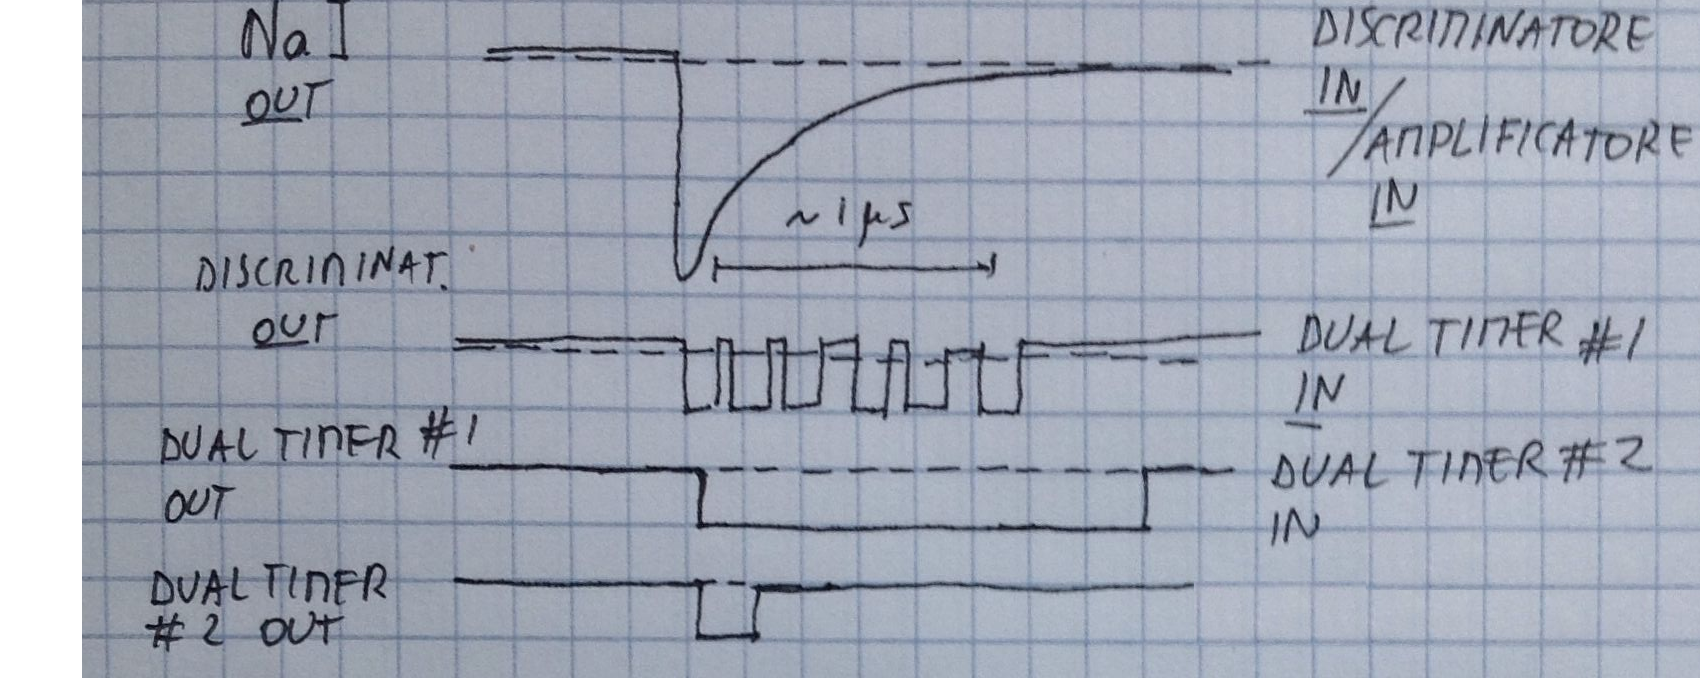
\includegraphics[scale=0.25]{dual_1}
\caption{Schema della digitalizzazione del segnale proveniente dallo scintillatore inorganico.}
\label{fig:dual_1}
\end{center}
\end{figure}

\begin{itemize}
	\item Invio dell'output del NaI al modulo di discriminazione. A causa dell'elevata ampiezza e durata dei segnali in uscita dal NaI, il discriminatore ha per output non uno, ma un treno di segnali digitali della durata selezionata sino a quando il segnale analogico non passa sotto soglia.
	\item Il treno di segnali viene mandato come input ad un modulo dual timer che restituisce un unico segnale digitale di durata impostata compatibile con la durata del segnale analogico.
	\item Il segnale così generato viene inviato come input ad una seconda unità di dual timing al fine di ottenere a partire da esso un segnale digitale dalla durata dell'ordine delle decine di nanosecondi in coincidenza con la fase di salita del segnale dell'inorganico.
\end{itemize}

\subsection{Scheda di acquisizione e software}
Ogni segnale analogico\footnote{In realtà in determinate condizioni, come si vedrà successivamente, non vengono acquisiti tutti i segnali ma solo quelli per cui un segnale di gate è attivo.} proveniente dallo scintillatore inorganico viene analizzato da una scheda di acquisizione, che provvede ad attribuirgli un determinato canale (da 0 a 8192) a seconda della sua ampiezza. I risultati vengono memorizzati e rappresentati in forma di istogramma da un software, che può in seguito salvare in formato ASCII gli spettri così ottenuti per una successiva analisi. 


\section{Operazioni preliminari}

\subsection{Stima della dose}



\subsection{Determinazione del punto di lavoro degli scintillatori}
Prendendo in considerazione lo scintillatore plastico, si è in primo luogo tracciata la curva dei conteggi in funzione della tensione di alimentazione. \\
Osservando l'assenza di una qualsivoglia struttura di plateau, si è effettuata un'analisi separata del rumore riposizionando lo scintillatore plastico in una zona del tutto schermata dal fascio principale. \\ 
Alla tensione di alimentazione di $ 1700V$ e con $ 50 mV$ di tensione di soglia (valore minimo consentito) si è osservato¸in un tempo di misura di 10s il seguente rapporto tra conteggi:
\begin{equation}
\frac{N-noise}{N-fascio}=\frac{216}{64316}=0.0033
\end{equation}
dell'ordine dell'incertezza statistica sui conteggi in presenza di sorgente. \\
Essendo dunque nel range di tensione di alimentazione suggerito trascurabile la frazione di eventi di rumore, ci si attende che la curva di alimentazione si mantenga crescente saturando eventualmente a tensioni sopra le quali tutti i segnali prodotti nello scintillatore vengono amplificate dal PMT in un segnale sopra la soglia di discriminazione. \\
Un discorso analogo è valido anche per lo scintillatore inorganico, per il quale la saturazione dei conteggi è particolarmente visibile. L'operazione è stata effettuata allineando lo scintillatore con il collimatore del fascio.[INSERIRE IMMAGINE]\\
Al fine di assicurarsi della legittimità degli eventi conteggiati in tale fase è stata effettuata una stima degli eventi attesi sullo scintillatore inorganico nota l'attività della sorgente.
Il calcolo assume un'efficienza di rivelazione dell'apparato coinvolto dell'ordine dell'unità, e si riduce alla stima del numero di fotoni emessi dalla sorgente (assunta isotropa l'emissività di quest'ultima) nella porzione dell'angolo solido individuata dal canale di collimazione, del quale sono noti lunghezza e larghezza. Si ottiene: \\
\begin{equation}
(\frac{dN}{dt})_{est.}\simeq 2.5\cdot 10^{4} evts./s \ \ \ \ (\frac{dN}{dt})_{mis.}=2.75\cdot 10^{4} evts./s
\end{equation}


\subsection{Caratteristiche geometriche del fascio} \label{subsec:geom_fascio}
\'E necessario studiare l'estensione angolare del fascio per stimare correttamente l'errore sulla lettura dell'angolo (sez. \ref{subsec:err_angolo}) e per poter correttamente interpretare i risultati successivi. Per fare ciò si è rimosso lo scintillatore plastico dal sistema e si è studiato l'andamento dei conteggi dello scintillatore inorganico in funzione della sua posizione angolare. Il risultato è mostrato in fig.!!!REF!!!.

%\includegraphics[width\textwidth]{•}

La curva risulta essere ben descritta da una gaussiana, con parametri:
\begin{equation}
\mu = ...°
\nonumber
\end{equation}
\begin{equation}
\sigma = ...°
\nonumber
\end{equation}


L'asimmetria rispetto a $\theta = 0°$ determina la necessità di traslare le future misure angolari di una quantità $\mu$.


\subsection{Stima dell'incertezza sull'angolo} \label{subsec:err_angolo}
La misura della posizione angolare dello scintillatore inorganico è soggetta ad un'incertezza legata sia alla lettura, ovvero alla capacità dell'occhio di individuare il centro dello scintillatore, sia alla distanza tra la proiezione del punto di interazione sul piano del goniometro e il centro del goniometro stesso.
\subsubsection{Incertezza sulla lettura}

Una prima fonte di errore sulla lettura dell'angolo sono rappresentate dalla limitata capacità da parte dell'occhio umano di valutare l'allineamento tra lo scintillatore e l'indicatore dell'angolo sul goniometro. Si è stimata l'incertezza così introdotta in $0.1°$ effettuando più volte operazioni fittizie di allineamento e verificando di volta in volta l'errore angolare commesso.

\subsubsection{Incertezza sul punto di interazione}
Questo tipo di incertezza, come si vedrà in sez.!!!! non si riflette in un effettivo errore sull'angolo, in quanto influisce solamente sulla forma dello spettro in energia osservato e viene dunque incluso nell'errore delle misure di energia.  \\
\vspace{0.8 cm}
Calcoli teorici\cite{compton_total} forniscono il valore della sezione d'urto Compton totale:

\begin{equation}
\sigma = 3.7 \cdot 10^{-25} cm^2
\nonumber
\end{equation}

Considerando l'energia media della sorgente utilizzata (Cobalto, $E/m_e = 2.45$) gli urti possono essere considerati avvenenti tra fotoni ed elettroni liberi. Considerata anche la densità di un polimero tipico (circa $1 g/cm^3$) e il fatto che l'elemento preponderante in questi materiali è il carbonio (in cui metà della massa è dovuta a protoni) è possibile stimare la densità numerica di elettroni, da cui il libero cammino medio di un fotone: \\
 
\begin{equation}
\lambda = \frac{1}{n_{elettroni} \cdot \sigma} = \frac{m_{protone}}{\frac{1}{2} \cdot \rho \cdot \sigma} \approx 10 \ cm
\nonumber
\end{equation}

Essendo questa misura un fattore quasi 10 maggiore dello spessore dello scintillatore plastico, è ragionevole supporre che la probabilità di interazione sia costante lungo lo spessore dello scintillatore. La non conoscenza del punto di interazione porta ad un errore sulla lettura dell'angolo, come è schematizzato in fig.!!!REF!!!. 

%\includegraphics[width=\textwidth]{""} \label{fig:err_angolo}

Si può calcolare:
\begin{equation}
\Delta \alpha_v = \frac{\Delta h_v}{L} sin\alpha
\nonumber
\end{equation}

Il punto di interazione non è determinato anche a causa dell'estensione del fascio stesso (sez. \ref{subsec:geom_fascio}). Questo si traduce in un'incertezza sull'angolo che può essere espressa matematicamente in modo analogo alla precedente:

\begin{equation}
\Delta \alpha_o = \frac{\Delta h_o}{L} cos\alpha
\nonumber
\end{equation}

Tuttavia una rapida stima permette di dimostrare che quest'ultimo produce un effetto trascurabile rispetto al precedente. Come è stato misurato in sez. \ref{subsec:geom_fascio}, il fascio ha una distribuzione ben descritta da una gaussiana con $\sigma = 3.97 °$. Sapendo la distanza tra lo scintillatore inorganico e quello plastico (sez. \ref{sec:apparato}) si trova, con metodi geometrici, che il segmento intercettato dal fascio sullo scintillatore plastico misura \\
\begin{equation}
\Delta h_o \approx 0.5 mm
\end{equation}

da cui si può ricavare \\

da confrontare con il $\Delta \alpha_v$ ottenuto utilizzando $\Delta h_v = 0.72 \ cm$, corrispondente alla deviazione standard di una distribuzione uniforme di ampiezza uguale allo spessore dello scintillatore plastico. Essendo l'errore approssimativamente lineare in $\Delta h$ risulta che: \\
\begin{equation}
\frac{\Delta \alpha_o}{\Delta \alpha_v} = \frac{\Delta h_o}{\Delta h_v} = 0.07 
\end{equation}

e dunque trascurabile.

Un'altra fonte di errore è quella dovuta all'estensione del rivelatore stesso, che occupa una porzione angolare calcolabile, una volta nota la configurazione geometrica, di \\
\begin{equation}
\Delta \alpha = \frac{5.08}{30} rad = 9.7°
\nonumber
\end{equation}





\subsection{Calibrazione dello scintillatore inorganico}

Essendo lo scintillatore inorganico in grado di produrre un segnale di output proporzionale all'energia in esso depositata dai prodotti, è necessaria un'operazione di calibrazione per determinare la legge che associ a ciascun canale dell'analizzatore la corrispondente energia rilasciata nello scintillatore. 
Per fare ciò si è fatto uso di quattro sorgenti di piccola intensità per le quali sono ben note a priori le energie dei fotoni emessi nel decadimento:

[TABELLA CON SORGENTI E PICCHI]

Onde minimizzare la contaminazione da parte dei fotoni emessi dalla sorgente principale, la procedura è stata effettuata ponendo lo scintillatore inorganico ad un angolo di circa $90°$ dalla direttrice del fascio, ponendo inoltre degli appositi schermi in piombo tra la sorgente primaria e il rivelatore. Vista la scarsa intensità delle sorgenti di calibrazione, queste ultime sono state poste direttamente a contatto con il rivestimento in alluminio in modo tale da massimizzare la frazione di angolo solido coperto dal rivelatore.\\
(ERRORI SULLA POSIZIONE)\\
Gli spettri così ottenuti grazie all'analizzatore multicanale sono visualizzati e salvati sotto forma di istogramma, rendendo così possibile l'estrazione della posizione in canali dei picchi mediante un fit gaussiano degli stessi. La legittimità del fit gaussiano deriva dalla monocromaticità delle sorgenti. In seguito tuttavia agli errori sperimentali collegati al processo di rivelazione e al rumore introdotto nella catena di lettura, la distribuzione ideale a delta di Dirac si manifesta come una Gaussiana con una determinata FWHM.\\

Dati i punti disponibili, non è stato osservato un andamento lineare per la curva di calibrazione. Si è pertanto proceduto con un fit polinomiale di grado superiore.\\
Al fine di determinare il grado del migliore fit , si è verificato il più piccolo grado per cui il coefficiente del polinomio risultato del fit è compatibile con zero. Quando ciò accade il coefficiente in questione sarà distribuito come una \cite{delprete_normalreg} Normale a media 0 e varianza ignota $\sigma$ :
\begin{equation}
a_{r}\ \sim \  N(0,\sigma) \ \ \ \rightarrow \ \ \  \dfrac{a^2_{r}}{\sigma^2}\ \sim\ \chi^2_{1} 
\nonumber
\end{equation}
Dove $r$ rappresenta il numero di parametri stimati attraverso il fit polinomiale. Il grado del polinomio utilizzato è pertanto $r-1$. Si procede testando di volta in volta per vari valori di $r$ l'ipotesi nulla di compatibilità con zero del coefficiente del grado massimo. Non essendo nota la varianza sui parametri, ma solo la sua stima prodotta dal fit, il test è da eseguirsi sulla distribuzione Fisher-Snedecor \cite{delprete_normalreg}:
\begin{equation}
f\ = \ \frac{a_r^2}{s^2}\ = \ \frac{\chi^2_{r-1}-\chi^2_r}{\chi^2_r}\ \sim \ F_{1;n-r-1}
\nonumber
\end{equation}
Nella quale $n$ rappresenta il numero di punti sperimentali su cui il fit è effettuato. Tale metodo non permette tuttavia di testare il coefficiente del quinto grado, per il quale il numero di gradi di libertà della distribuzione Fisher-Snedecor si riduce a zero. Ci si è pertanto limitati a effettuare i test d'ipotesi per $R<6$. In tabella sono riportati i valori delle variabili statistiche calcolate al fine di ottenere il P-Value corrispondente a ciascuna ipotesi nulla.\\

\subsubsection{Contributo all'incertezza sull'energia}

L'incertezza sull'energia è ricavata simulando un determinato numero di esperimenti secondo lo schema:
\begin{enumerate}
\item Generazione per ogni pseudoesperimento della posizione in canali dei picchi di emissione delle sorgenti di calibrazione secondo una distribuzione gaussiana con valor medio e varianza uguali ai rispettivi valori misurati sperimentalmente.
\item Fit dei punti così generati utilizzando sempre un polinomio di terzo grado.
\item Canale per canale si è costruito un istogramma dei valori dell'energia ad esso corrispondente ottenuta in ciascuno degli pseudoesperimenti.
\item Estrazione, canale per canale, della media e dello stimatore della varianza della distribuzione così tracciata.
\end{enumerate}

La banda di incertezza sulla curva di calibrazione e le incertezze assolute in funzione dell'energia sono mostrate nelle figure \ref{fig:calib_en} e \ref{fig:err_en}.

\begin{figure}[h!] 
\includegraphics[width=\textwidth]{"calibrazione2"}
\caption{...}
\label{fig:calib_en}
\end{figure}

\begin{figure}[h!] 
\includegraphics[width=\textwidth]{"err_en4"}
\caption{...}
\label{fig:err_en}
\end{figure}


\section{Metodo di misura}
\subsection{Determinazione di $m_e$ dal fit della relazione Energia-Angolo}
La procedura sperimentale consiste semplicemente nell'acquisizione delle misure di spettro da parte dello scintillatore inorganico a diversi angoli di scattering, misurando di volta in volta l'energia corrispondente al fotopicco. La relazione su cui verrà effettuato il fit è quella descritta in sez. \ref{sec:intro} (eq. \ref{eq:en_ang}).
\subsection{Segnale di gate} \label{subsec:gate}
Al fine di ridurre il rapporto segnale/rumore nelle misure di spettro [solo in queste???] si sfrutta la modalità di acquisizione con gate dell'analizzatore multicanale. Tale segnale si costruisce a partire dalla coincidenza tra gli output dei due scintillatori. In tale modo si ordina l'acquisizione del segnale in output dell'inorganico solamente se viene rivelato in coincidenza temporale ad esso un evento nello scintillatore plastico, idealmente dovuto all'elettrone rinculante.
\\
Il segnale in ingresso al gate deve essere conforme per durata al segnale di input all'analizzatore, a sua volta in uscita dal sistema di amplificazione-shaping. Per generare un segnale di questo tipo si è proceduto in questo modo:

!!!CORREGGERE PERCHE GIA MESSO NELL APPARATO SPERIMENTALE!!!
\begin{itemize}
	\item Invio dell'output del NaI al modulo di discriminazione. A causa dell'elevata ampiezza e durata dei segnali in uscita dal NaI, il discriminatore ha per output non uno, ma un treno di segnali digitali della durata selezionata sino a quando il segnale analogico non passa sotto soglia.
	\item Il treno di segnali viene mandato come input ad un modulo dual timer che restituisce un unico segnale digitale di durata impostata compatibile con la durata del segnale analogico.
	\item Il segnale così generato viene inviato come input ad una seconda unità di dual timing al fine di ottenere a partire da esso un segnale digitale dalla durata dell'ordine delle decine di nanosecondi in coincidenza con la fase di salita del segnale dell'inorganico.
	\item Il segnale viene inviato al modulo di coincidenza con l'output digitalizzato del plastico.
	\item L'output della coincidenza è inviato in input ad una terza unità dual timer al fine di ottenere un segnale della stessa durata del segnale dello scintillatore inorganico amplificato e formato.
\end{itemize}

L'efficacia del metodo di acquisizione con gate dipende però fortemente dalla rivelabilità dell'elettrone rinculante, e sarà pertanto massimamente efficacie ad angoli di diffusione alti, per i quali l'energia cinetica trasferita è massima. \\
A piccoli angoli di diffusione, per contro, l'efficienza del gate risulta ampiamente ridotta, al punto da rendere la procedura completamente inefficace. [MAGARI IMMAGINE GATE NO GATE STESSO ANGOLO]. Ci si è pertanto limitati ad sfruttare il segnale di gate per angoli di diffusione $|\alpha|>30°$. 

\subsubsection{Caratteristiche degli spettri}
Nelle figure [1 e 2!!!!!!!!!!!!!!!!!!!] sono mostrati gli spettri ottenuti nelle due diverse modalità di acquisizione posizionando lo scintillatore inorganico ad un angolo di 30° sulla destra dello zero del goniometro. \\
Lo spettro acquisito senza l'ausilio del gate presenta due picchi marcati in corrispondenza delle energie dei fotoni primari emessi dalla sorgente. Se ne deduce che per angoli uguali o inferiori a 30° il numero di fotoni che penetra la schermatura della sorgente venendo così rivelata nell'inorganico è superiore al numero di eventi legittimi rivelati dall'inorganico in seguito ad un'interazione Compton nello scintillatore plastico.
La [figura2!!!!!!!!!!!!!!!] mostra come l'acquisizione in modalità GATE permetta di ridurre drasticamente il fondo di fotoni diretti, come deducibile dal rapporto tra le ampiezze tra i fotopicchi (non risolti) e i picchi, appena accennati, di fascio diretto. Si nota inoltre che in entrambe le figure i picchi imputati al fascio diretto non si trovano nella posizione teorica ($1.17 \ MeV e 1.33 \ MeV$) ma sono spostati verso il basso. Questo effetto è stato interpretato con il fatto che, affinché i fotoni provenienti dalla sorgente possano arrivare allo scintillatore inorganico ad angoli alti rispetto alla divergenza angolare del fascio devono attraversare parte della schermatura e perdere quindi parte della loro energia. \\
Nello spettro ottenuto con l'ausilio del gate è inoltre ben distinguibile la \textit{spalla Compton}\footnote{Come si vedrà in sez. \ref{subsec:spalla}, tuttavia, la spalla Compton presenta una traslazione rispetto al picco indicato in Fig. \ref{fig:spettro_gate}.}, dovuta agli eventi Compton ad angolo massimo all'interno dello scintillatore inorganico. Un elemento analogo è ravvisato anche nella [figura1], per quanto in questo caso esso sia dovuto agli eventi di backscattering nell'inorganico causati dai fotoni di fascio diretto, in maggioranza.\\
L'intervallo di energie dei fotoni Compton nel presente esperimento comprende l'energia di soglia sopra la quale è possibile la produzione di coppia $e^+\ e^-$. Ciononostante, alle energie dell'esperimento le sezioni d'urto di produzione e Compton stanno nel seguente rapporto:
\begin{equation}
\frac{\sigma_{pair}}{\sigma_{compt}}\simeq 10^{-2}
\end{equation}
Il che giustifica la non visibilità dei tipici picchi a $E_\gamma \ - \ m_e c^2$ e $E_\gamma \ - \ 2m_e c^2$ dovuti alla fuga di uno o entrambi i fotoni da $511 keV$ prodotti nell'annichilazione del positrone proveniente dall'evento di produzione di coppia.\\
Attenendosi sempre allo spettro con gate [immag!!!!!2], si osserva una struttura complessa a energie di circa $200 keV$. Essa è dovuta al gran numero di fotoni primari che subiscono un'interazione Compton a $\theta \ \simeq \ 180°$ nel materiale di schermo in prossimità della sorgente per poi fuoriuscire dal vano, subire un'interazione Compton nel plastico ed essere rivelati infine nello scintillatore inorganico. L'energia di questi fotoni è circa:

\begin{equation}
E'\ \simeq \ \frac{E}{1+\frac{2E}{m_e}} \ = \ 210\ \emph{keV}
\end{equation}

I fotoni in questione vengono rivelati nello scintillatore inorganico tramite i medesimi processi che interessano i fotoni primari, e risulteranno dunque in una struttura spettrale analoga, con fotopicchi, spalla e continuo Compton difficilmente risolvibili. \\
%RIMUOVERE!!!!!![Il fatto che lo spettro di backscattering si trovi a energie costanti con l'angolo è giustificabile con il fatto che la relazione energia-angolo per un fenomeno compton con energia primaria E generica ha pendenza proporzionale a E quadro. Pertanto la pendenza sarà 0.04 .]RIMUOVEREEEEEEE

A energie di circa $75 \ keV$ si trova inoltre uno stretto picco compatibile con i \textit{raggi X} molli emessi per fluorescenza dal piombo contenuto nell'apparato di schermo. \cite{X_Ray}

\subsubsection{Risoluzione dei fotopicchi}
La capacità di distinguere due fotopicchi è legata alla differenza di energia tra i picchi dei fotoni diffusi ad un dato angolo. Si è dunque ricavata la relazione algebrica che lega la suddetta differenza alle energie dei fotoni emessi dalla sorgente e all'angolo di misura. 

\begin{figure}
\includegraphics[width=\textwidth]{"distanza_picchi"}
\caption{Differenza di energia tra i picchi dei fotoni diffusi del Cobalto in funzione dell'angolo di misura}
\label{fig:dist_picchi}
\end{figure}

Come si può vedere in Fig. \ref{fig:dist_picchi} la differenza di energia tra i fotopicchi tende a diminuire, rendendo sempre più difficile risolverli all'aumentare dell'angolo di misura. La risolvibilità dipende infatti dal rapporto tra questa quantità e le FWHM dei singoli picchi. Nella maggior parte dei casi non si è riusciti a risolvere i due fotopicchi (sez. \cite{subsec:picchi}), per cui è stato deciso di procedere come segue:

\begin{enumerate}
\item Se la forma dello spettro misurato è significativamente diversa da una gaussiana è stato eseguito un fit \textit{bigaussiano} ed è stata estratta la media aritmetica dei picchi.
\item Se la forma dello spettro misurato è compatibile con quella di una gaussiana è stato estratto il valore del massimo locale.
\end{enumerate}

Ad angoli sufficientemente alti, in cui la differenza di energia tra i picchi è minore, si verifica la seconda condizione. In questo caso l'energia misurata è circa uguale alla media tra i fotopicchi (l'intensità di emissione delle due righe da parte della sorgente è circa la stessa). A rigore, dunque, non è legittimo utilizzare, nella relazione \eqref{eq:en_ang}, i fotopicchi misurati, poiché in generale \\
\begin{equation}
\frac{E'(\theta,E_1) + E'(\theta,E_2)}{2} \neq E'(\theta, \frac{E_1+E_2}{2})
\end{equation}

Tuttavia è stato verificato che i due membri sono uguali entro un errore del $0.1 \ \%$, che è in ogni caso trascurabile rispetto all'errore sull'energia

\subsection{Distanza tra la \textit{spalla Compton} e i fotopicchi}
[VEDERE SE INTRODUZIONE] Assumendo che i fotoni in ingresso al rivelatore posseggano la medesima energia e che essi vi subiscano al massimo una sola interazione, la situazione in cui è massima l'energia trasferita al reticolo del cristallo senza che avvenga effetto fotoelettrico è quella in cui il fotone interagisca Compton con angolo di diffusione $theta_2 \ = \ 180°$. Sotto questi assunti, dunque, lo spettro continuo Compton misurato decresce rapidamente all'approssimarsi dell'end point, il quale è dato da:
\begin{equation}
E_{CE} \ = E' \ \ - \ \frac{E'(\theta_1)}{1+\frac{2E'(\theta_1)}{m_e}}     \nonumber
\end{equation}
Dove $\theta_1$ rappresenta l'angolo con cui avviene la prima diffusione Compton nello scintillatore plastico, risultante nei fotoni in ingresso all'inorganico con energia $E'$.
La distanza tra i fotopicchi e spalla Compton è dunque funzione \textit{decrescente} dell'angolo a cui viene posto il rivelatore rispetto all'asse del fascio.\\
La regione di spettro, idealmente vuota, tra spalla Compton e fotopicchi è in realtà occupata da un fondo di eventi dovuto a più di una interazione Compton nel NaI , per i quali l'energia massima depositata può eccedere il limite massimo della singola interazione. 
Questo effetto, unitamente all'allargamento sperimentale degli spettri, che risulta in una coda a destra della spalla, rende la determinazione della posizione della spalla Compton relativamente ai fotopicchi un'operazione non sempre immediata. \\
Il fit della distanza in funzione dell'angolo con la relazione teorica può portare ad una seconda stima della massa dell'elettrone, sebbene non indipendente rispetto alla stima effettuata fittando la sola relazione energia-angolo.


\section{Klein-Nishina}

\section{Risultati sperimentali}
\subsection{Misura dei picchi} \label{subsec:picchi}



\section{Conclusioni}
Fare il mea culpa sulla determinazione del punto di lavoro dell'inorganico che si poteva in qualche modo cercare un'alimentazione per la quale era minima l'analisi della FWHM, poi distanza tra scintillatore plastico e sorgente.

note:
spiegare bene errore sull'angolo, coincidenze casuali trascurabili, visto effetto dello shift picchetto-spalla Compton anche in naicat.pdf in vari spettri (Promezio, Vanadio, Manganese).

\input{bibcompton.bib}


\end{document}
